\section{przypadek testowy 2}
\subsection{Cel: }
Celem badania jest sprawdzenie czy rzeczywista złożoność czasowa dla algorytmu k-random jest zgodna z oczekiwanym \(O(n)\).
\subsection{Założenia: }
Podczas badania korzystać będziemy z losowych instancji grafów pełnych, symetrycznych o \(n \in \{ 100, 200, 300 \ldots 1000 \}\) wierzchołkach oraz ustalonym \( k = 1000 \). Badanie czasu każdego rozmiaru grafów zostało powtórzone 100 razy.

\subsection{Wyniki: }
\nameref{table_1} przedstawia czasy wykonania programu. Dane w tabach, dla czytelności, zostały zaokrąglone do 3 miejsc po przecinku. W dalszych obliczeniach korzystaliśmy z danych dokładnych zamieszczonych w pliku csv/xlsx.
\begin{table}[!ht]
  \centering
  \begin{tabular}{|c|c|c|c|c|c|c|c|c|c|c| p{10cm} }
  \hline
      n & 100 & 200 & 300 & 400 & 500 & 600 & 700 & 800 & 900 & 1000 \\ \hline \hline
      T [s] & 0.781 & 0.810 & 0.860 & 0.903 & 0.922 & 0.957 & 0.996 & 1.007 & 1.044 & 1.074 \\ \hline
      SD & 0.009 & 0.010 & 0.223 & 0.033 & 0.037 & 0.028 & 0.029 & 0.020 & 0.020 & 0.012 \\ \hline
      SE & 0.001 & 0.001 & 0.022 & 0.003 & 0.004 & 0.003 & 0.003 & 0.002 & 0.002 & 0.001 \\ \hline
  \end{tabular}
  \caption{T - średni czas wykoniania (w sekundach), SD - odchylenie standardowe, SE - błąd standardowy}
\end{table}

Odchylenie standardowe oraz błąd standardowy zostały obliczone według wzorów: \\
\begin{equation} \label{eq:1}
  \sigma = \sqrt{\frac{\sum_{n = 1}^{100}(\bar{x} - x_n)^2}{100}}
\end{equation}
  
odchylenie standardowe~\ref{eq:1}

\begin{equation} \label{eq:2}
  \sigma_{\bar{x}} = \frac{\sigma}{\sqrt{100}}
\end{equation}
  
błąd standardowy \ref{eq:2} 

\subsection{Wykresy: }
\begin{figure}[h]
    \centering
    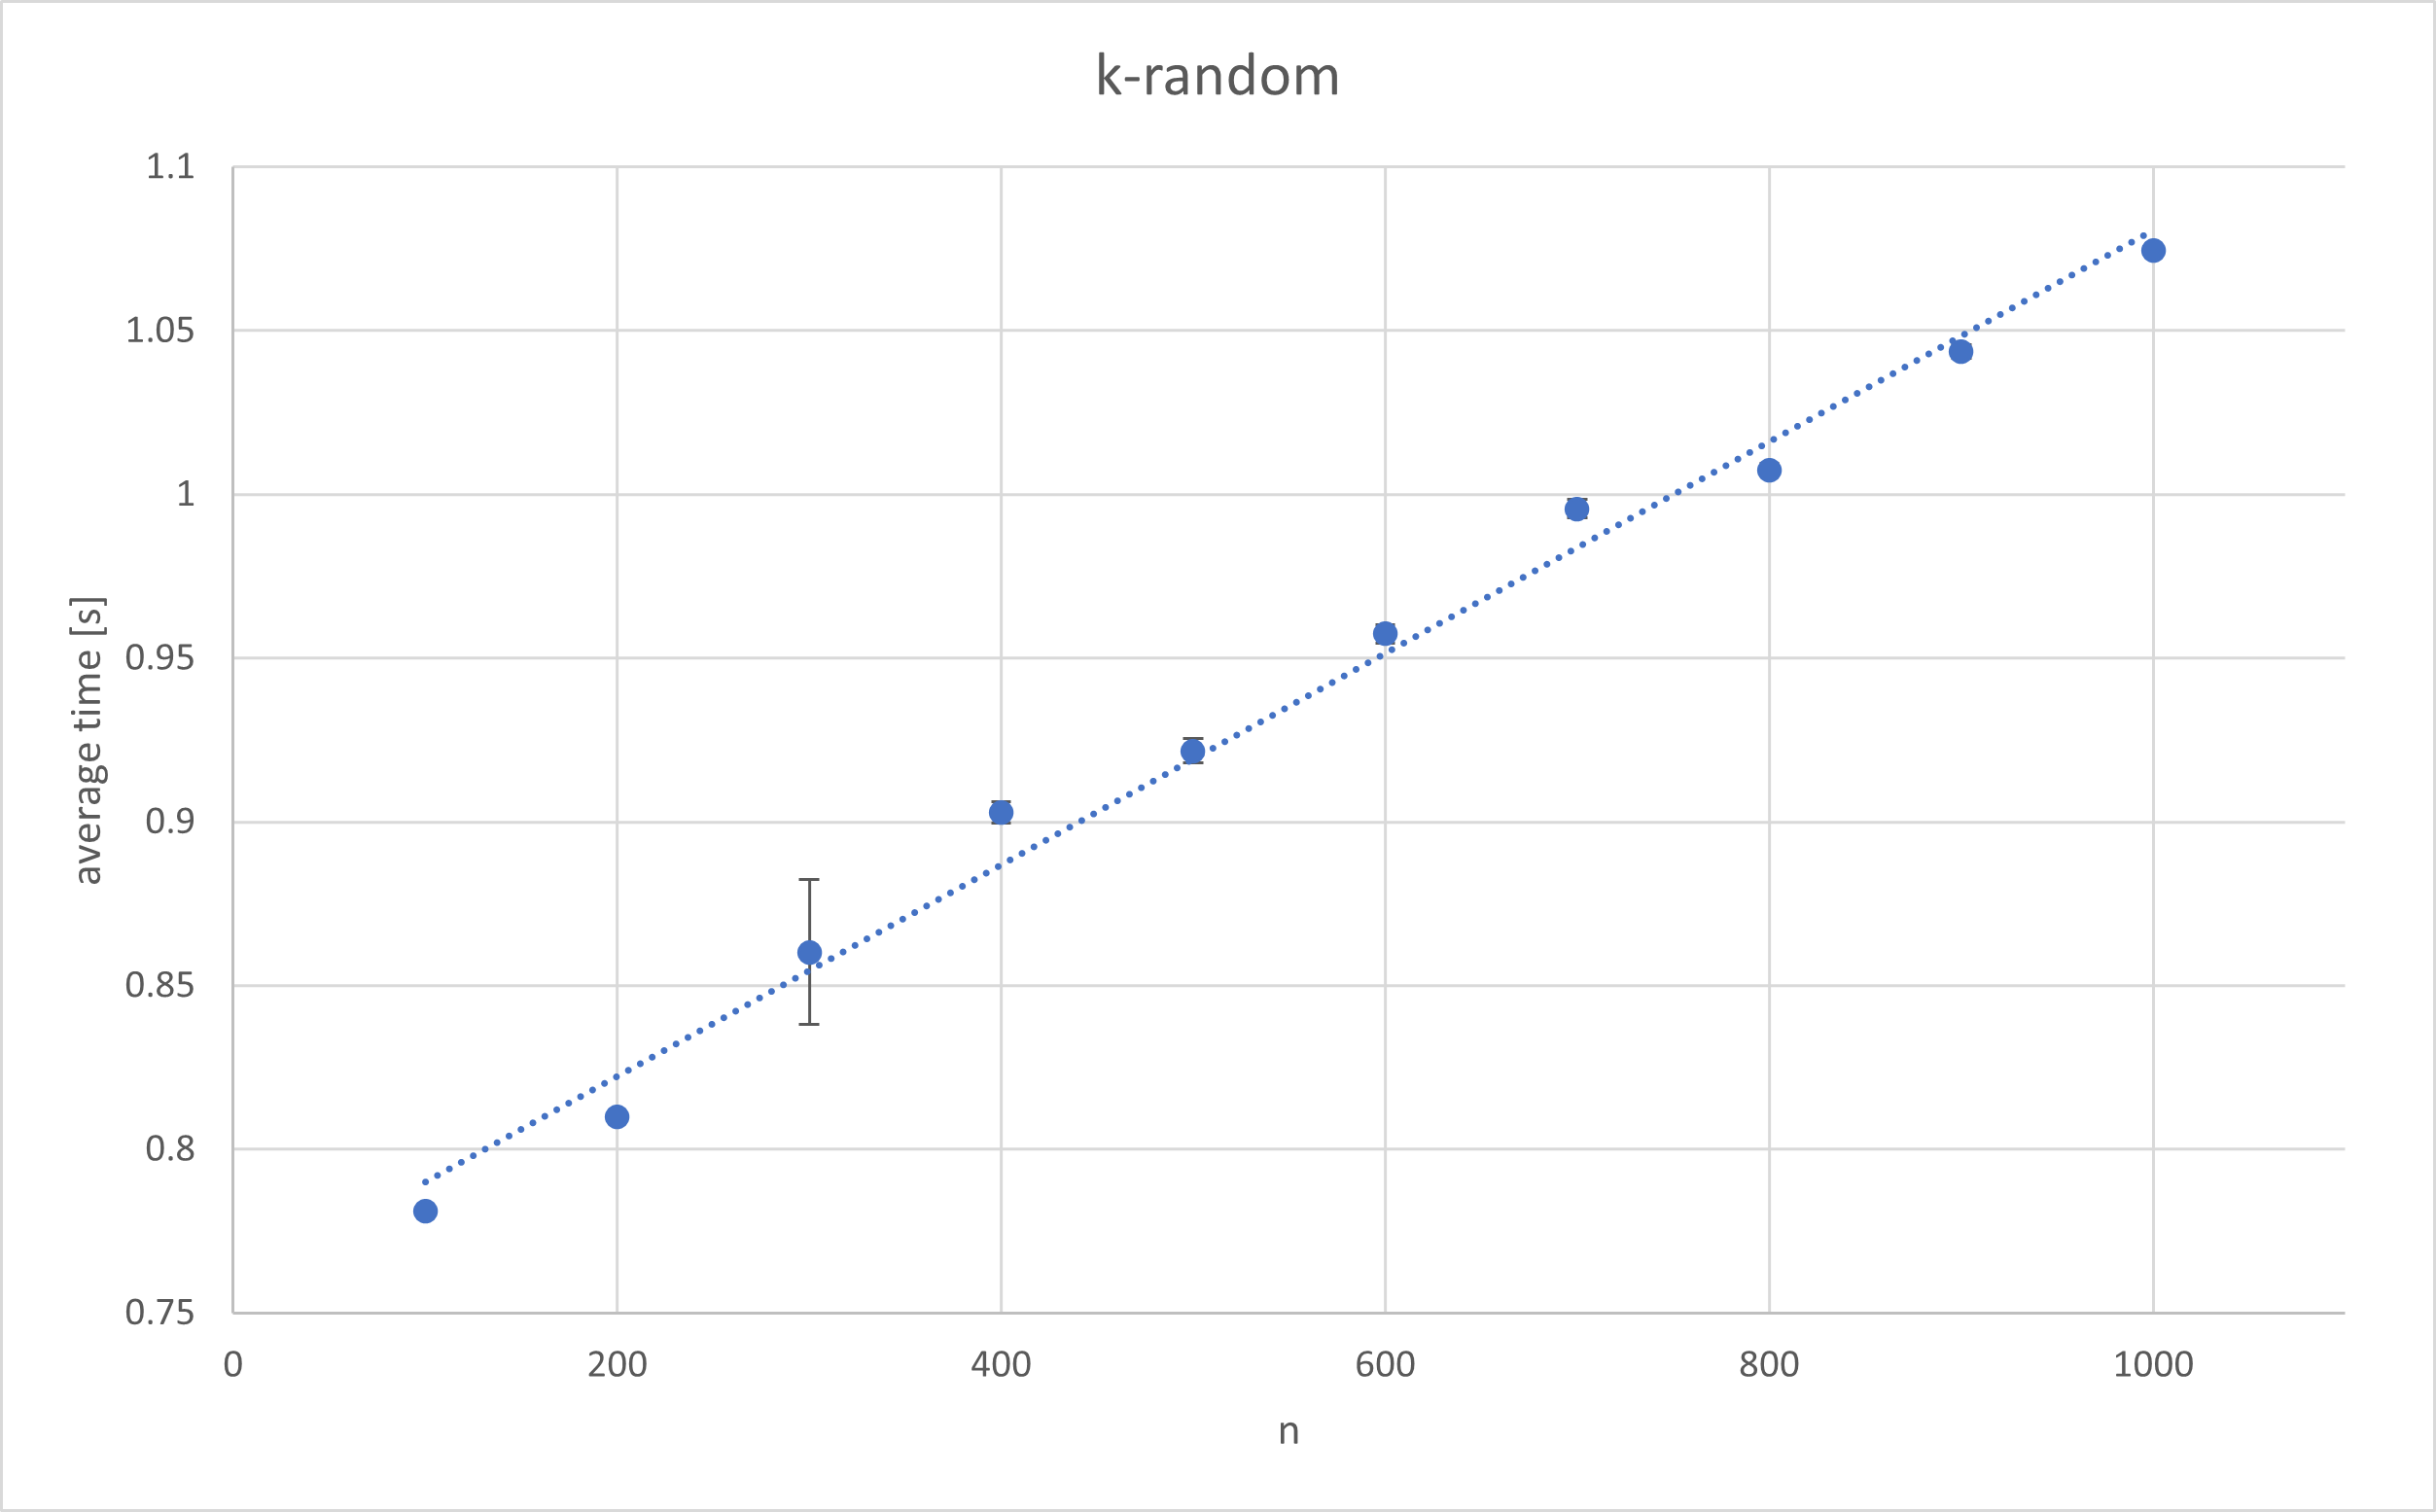
\includegraphics[width=\linewidth]{chart_test1.png}
    \caption{średnie czasy wykonania wraz z błędami standardowymi}
\end{figure}
Na osi OX wykresu naniesione zostały \(n\) dla których wykonywany był pomniar, na osi OY uśrednione wartości czasów wykonania wraz z zaznaczonymi błędami standardowymi.
Zauważyć można że punkty wskazujące średnie czasy wykonania ustaiwione są w zależności liniowej.


\subsection{Wnioski: }
Zmierzone dane potwierdziły tezę, że złożoność czasowa metody k-random przy ustalonym k jest liniowa względem wielkości grafu. 

\subsection{Tabela czasów: }
\begin{table}[!ht]
  \centering
  \begin{tabular}{|c|c|c|c|c|c|c|c|c|c|}
  \hline
      100 & 200 & 300 & 400 & 500 & 600 & 700 & 800 & 900 & 1000 \\ \hline \hline
      0.791 & 0.803 & 0.855 & 0.975 & 0.895 & 0.921 & 1.063 & 1.008 & 1.028 & 1.073 \\ \hline
      0.776 & 0.819 & 0.831 & 0.961 & 0.937 & 0.921 & 1.020 & 1.006 & 1.032 & 1.081 \\ \hline
      0.790 & 0.810 & 0.836 & 0.934 & 0.963 & 0.946 & 1.026 & 1.019 & 1.044 & 1.076 \\ \hline
      0.783 & 0.817 & 0.836 & 0.942 & 0.945 & 0.971 & 1.038 & 1.000 & 1.033 & 1.080 \\ \hline
      0.788 & 0.808 & 0.834 & 0.932 & 0.935 & 0.917 & 1.022 & 1.025 & 1.039 & 1.062 \\ \hline
      0.783 & 0.803 & 0.841 & 0.929 & 0.938 & 0.942 & 1.022 & 1.011 & 1.032 & 1.090 \\ \hline
      0.784 & 0.815 & 0.843 & 0.926 & 0.898 & 0.930 & 1.042 & 1.007 & 1.034 & 1.105 \\ \hline
      0.780 & 0.806 & 0.829 & 0.968 & 0.892 & 0.921 & 1.025 & 1.006 & 1.036 & 1.099 \\ \hline
      0.781 & 0.813 & 0.853 & 0.955 & 0.918 & 0.909 & 1.033 & 0.999 & 1.016 & 1.082 \\ \hline
      0.786 & 0.800 & 0.838 & 0.936 & 0.918 & 0.922 & 1.030 & 1.003 & 1.039 & 1.091 \\ \hline
      0.778 & 0.805 & 0.850 & 0.912 & 0.953 & 0.931 & 1.028 & 1.009 & 1.036 & 1.075 \\ \hline
      0.786 & 0.811 & 0.833 & 0.954 & 0.961 & 0.922 & 1.027 & 1.004 & 1.031 & 1.091 \\ \hline
      0.772 & 0.812 & 0.836 & 0.866 & 0.898 & 0.925 & 1.027 & 0.994 & 1.054 & 1.079 \\ \hline
      0.784 & 0.810 & 0.834 & 0.856 & 0.886 & 0.941 & 1.035 & 0.993 & 1.027 & 1.080 \\ \hline
      0.784 & 0.812 & 0.846 & 0.862 & 0.917 & 0.943 & 1.032 & 1.000 & 1.023 & 1.095 \\ \hline
      0.785 & 0.803 & 0.833 & 0.873 & 0.949 & 0.936 & 1.022 & 1.000 & 1.030 & 1.071 \\ \hline
      0.793 & 0.812 & 0.840 & 0.862 & 1.006 & 0.946 & 1.063 & 1.019 & 1.021 & 1.093 \\ \hline
      0.789 & 0.797 & 0.825 & 0.868 & 1.000 & 0.922 & 1.070 & 0.993 & 1.034 & 1.084 \\ \hline
      0.781 & 0.807 & 0.839 & 0.859 & 1.034 & 0.918 & 1.038 & 0.996 & 1.039 & 1.061 \\ \hline
      0.793 & 0.856 & 0.842 & 0.872 & 1.051 & 0.955 & 1.028 & 1.021 & 1.032 & 1.094 \\ \hline
      0.768 & 0.799 & 0.837 & 0.868 & 1.032 & 0.986 & 1.034 & 1.010 & 1.039 & 1.097 \\ \hline
      0.790 & 0.839 & 0.834 & 0.871 & 0.974 & 0.944 & 1.040 & 1.012 & 1.036 & 1.078 \\ \hline
      0.785 & 0.810 & 0.833 & 0.863 & 0.921 & 1.006 & 1.033 & 1.007 & 1.047 & 1.105 \\ \hline
      0.775 & 0.815 & 0.841 & 0.863 & 0.927 & 1.010 & 1.031 & 0.993 & 1.034 & 1.066 \\ \hline
      0.786 & 0.800 & 0.840 & 0.863 & 0.921 & 0.939 & 1.035 & 0.994 & 1.030 & 1.079 \\ \hline
      0.781 & 0.821 & 0.842 & 0.892 & 0.913 & 0.948 & 1.019 & 1.016 & 1.025 & 1.078 \\ \hline
      0.785 & 0.814 & 0.829 & 0.935 & 0.974 & 0.944 & 0.971 & 1.026 & 1.026 & 1.079 \\ \hline
      0.797 & 0.812 & 0.816 & 0.915 & 0.988 & 0.972 & 0.975 & 1.033 & 1.040 & 1.078 \\ \hline
      0.790 & 0.799 & 0.843 & 0.932 & 0.947 & 0.949 & 0.982 & 1.067 & 1.027 & 1.066 \\ \hline
      0.775 & 0.861 & 0.831 & 0.876 & 0.933 & 0.998 & 0.969 & 1.020 & 1.026 & 1.075 \\ \hline
      0.780 & 0.792 & 0.833 & 0.872 & 0.937 & 0.950 & 0.958 & 1.005 & 1.025 & 1.073 \\ \hline
      0.776 & 0.812 & 0.827 & 0.887 & 0.908 & 0.950 & 0.971 & 0.986 & 1.032 & 1.075 \\ \hline
      0.788 & 0.813 & 0.831 & 0.870 & 0.964 & 0.933 & 0.969 & 0.976 & 1.040 & 1.094 \\ \hline
      0.785 & 0.797 & 0.832 & 0.916 & 0.976 & 0.902 & 0.962 & 1.035 & 1.034 & 1.073 \\ \hline
      0.783 & 0.814 & 0.840 & 0.900 & 0.944 & 0.945 & 0.979 & 1.004 & 1.040 & 1.078 \\ \hline
      0.768 & 0.814 & 0.829 & 0.906 & 0.915 & 0.966 & 0.964 & 1.010 & 1.034 & 1.070 \\ \hline
      0.769 & 0.812 & 0.831 & 0.896 & 0.960 & 0.911 & 0.980 & 1.041 & 1.066 & 1.066 \\ \hline
      0.789 & 0.808 & 0.836 & 0.910 & 0.956 & 0.932 & 0.974 & 1.009 & 1.050 & 1.074 \\ \hline
      0.779 & 0.807 & 0.831 & 0.905 & 0.977 & 1.009 & 0.964 & 0.977 & 1.031 & 1.073 \\ \hline
      0.783 & 0.799 & 0.829 & 0.933 & 0.912 & 0.993 & 0.982 & 1.010 & 1.029 & 1.074 \\ \hline
      0.780 & 0.808 & 0.833 & 0.918 & 0.943 & 0.975 & 0.971 & 1.004 & 1.033 & 1.062 \\ \hline
      0.767 & 0.802 & 0.830 & 0.941 & 0.925 & 0.994 & 0.973 & 0.982 & 1.028 & 1.080 \\ \hline
      0.793 & 0.815 & 0.841 & 0.912 & 0.957 & 1.005 & 0.968 & 1.039 & 1.090 & 1.092 \\ \hline
      0.786 & 0.807 & 0.832 & 0.927 & 0.923 & 0.973 & 0.970 & 0.990 & 1.045 & 1.075 \\ \hline
      0.778 & 0.815 & 0.832 & 0.938 & 0.928 & 1.012 & 0.986 & 0.988 & 1.051 & 1.064 \\ \hline
      0.767 & 0.812 & 0.833 & 0.937 & 0.943 & 1.014 & 0.981 & 0.980 & 1.038 & 1.086 \\ \hline
      0.788 & 0.815 & 0.827 & 0.925 & 0.956 & 1.027 & 0.960 & 1.041 & 1.035 & 1.069 \\ \hline
      0.780 & 0.815 & 0.838 & 0.871 & 0.927 & 1.000 & 0.963 & 1.000 & 1.022 & 1.083 \\ \hline
      0.778 & 0.818 & 0.844 & 0.869 & 0.971 & 1.004 & 0.983 & 1.044 & 1.022 & 1.070 \\ \hline
      0.788 & 0.806 & 0.830 & 0.910 & 0.943 & 0.998 & 0.966 & 0.965 & 1.019 & 1.084 \\ \hline
    \end{tabular}
    \label{table_1}
    \caption{tabela czasów}
  \end{table}

  \begin{table}[!ht]
    \centering
    \begin{tabular}{|c|c|c|c|c|c|c|c|c|c|}
      \hline
      100 & 200 & 300 & 400 & 500 & 600 & 700 & 800 & 900 & 1000 \\ \hline\hline
      0.776 & 0.806 & 0.833 & 0.902 & 0.939 & 1.008 & 1.017 & 1.020 & 1.018 & 1.062 \\ \hline
      0.773 & 0.808 & 0.839 & 0.885 & 0.911 & 0.998 & 0.972 & 0.974 & 1.037 & 1.068 \\ \hline
      0.794 & 0.803 & 0.837 & 0.885 & 0.895 & 0.989 & 0.969 & 0.996 & 1.041 & 1.080 \\ \hline
      0.775 & 0.817 & 0.844 & 0.890 & 0.917 & 0.949 & 0.967 & 0.981 & 1.029 & 1.067 \\ \hline
      0.774 & 0.812 & 0.841 & 0.901 & 0.938 & 0.963 & 0.970 & 0.994 & 1.022 & 1.077 \\ \hline
      0.766 & 0.806 & 0.835 & 0.905 & 0.920 & 0.945 & 0.972 & 0.977 & 1.025 & 1.072 \\ \hline
      0.796 & 0.807 & 0.826 & 0.929 & 0.896 & 0.945 & 0.976 & 0.968 & 1.067 & 1.077 \\ \hline
      0.774 & 0.791 & 0.830 & 0.893 & 0.903 & 1.003 & 0.980 & 0.975 & 1.066 & 1.071 \\ \hline
      0.793 & 0.821 & 0.828 & 0.914 & 0.871 & 1.015 & 0.976 & 0.967 & 1.029 & 1.061 \\ \hline
      0.765 & 0.799 & 0.824 & 0.952 & 0.892 & 0.999 & 0.969 & 1.007 & 1.020 & 1.088 \\ \hline
      0.791 & 0.799 & 0.837 & 0.956 & 0.867 & 0.973 & 0.982 & 1.015 & 1.047 & 1.069 \\ \hline
      0.778 & 0.813 & 0.843 & 0.953 & 0.878 & 0.947 & 0.965 & 0.985 & 1.050 & 1.060 \\ \hline
      0.782 & 0.808 & 0.841 & 0.948 & 0.887 & 0.965 & 0.966 & 1.010 & 1.026 & 1.057 \\ \hline
      0.774 & 0.797 & 0.841 & 0.947 & 0.872 & 0.952 & 0.970 & 1.031 & 1.026 & 1.069 \\ \hline
      0.781 & 0.819 & 0.839 & 0.894 & 0.877 & 0.960 & 0.976 & 0.970 & 1.094 & 1.059 \\ \hline
      0.784 & 0.802 & 0.836 & 0.869 & 0.894 & 0.948 & 0.975 & 1.029 & 1.047 & 1.083 \\ \hline
      0.782 & 0.818 & 0.849 & 0.878 & 0.908 & 0.956 & 0.970 & 1.053 & 1.044 & 1.071 \\ \hline
      0.781 & 0.811 & 0.843 & 0.877 & 0.900 & 0.961 & 0.963 & 1.049 & 1.028 & 1.061 \\ \hline
      0.805 & 0.821 & 0.843 & 0.861 & 0.926 & 0.954 & 0.969 & 1.056 & 1.042 & 1.061 \\ \hline
      0.776 & 0.803 & 0.828 & 0.871 & 0.902 & 0.974 & 0.980 & 1.013 & 1.050 & 1.058 \\ \hline
      0.797 & 0.804 & 0.834 & 0.909 & 0.904 & 0.968 & 0.985 & 0.994 & 1.035 & 1.083 \\ \hline
      0.782 & 0.809 & 0.846 & 0.865 & 0.907 & 0.961 & 0.976 & 1.011 & 1.014 & 1.066 \\ \hline
      0.767 & 0.805 & 0.841 & 0.868 & 0.909 & 0.941 & 0.975 & 1.007 & 1.100 & 1.049 \\ \hline
      0.791 & 0.811 & 0.836 & 0.873 & 0.917 & 0.952 & 0.979 & 1.008 & 1.086 & 1.065 \\ \hline
      0.763 & 0.812 & 0.844 & 0.852 & 0.895 & 0.945 & 0.977 & 1.007 & 1.065 & 1.056 \\ \hline
      0.779 & 0.812 & 0.836 & 0.852 & 0.894 & 0.945 & 0.976 & 1.018 & 1.043 & 1.066 \\ \hline
      0.771 & 0.817 & 0.835 & 0.855 & 0.896 & 0.984 & 0.990 & 1.011 & 1.099 & 1.058 \\ \hline
      0.788 & 0.806 & 0.859 & 0.884 & 0.904 & 0.950 & 0.982 & 1.034 & 1.081 & 1.073 \\ \hline
      0.769 & 0.807 & 0.839 & 0.864 & 0.887 & 0.948 & 0.970 & 1.006 & 1.075 & 1.058 \\ \hline
      0.786 & 0.801 & 0.839 & 0.919 & 0.911 & 0.958 & 0.965 & 0.998 & 1.040 & 1.065 \\ \hline
      0.784 & 0.800 & 0.840 & 0.959 & 0.890 & 0.945 & 1.002 & 1.038 & 1.057 & 1.063 \\ \hline
      0.785 & 0.803 & 0.839 & 0.919 & 0.895 & 0.947 & 0.982 & 1.004 & 1.111 & 1.068 \\ \hline
      0.786 & 0.811 & 0.858 & 0.908 & 0.894 & 0.937 & 0.986 & 1.019 & 1.092 & 1.062 \\ \hline
      0.782 & 0.810 & 0.831 & 0.904 & 0.876 & 0.956 & 0.989 & 0.999 & 1.053 & 1.072 \\ \hline
      0.766 & 0.801 & 0.845 & 0.910 & 0.882 & 0.952 & 1.001 & 1.013 & 1.071 & 1.050 \\ \hline
      0.765 & 0.811 & 0.852 & 0.904 & 0.897 & 0.950 & 1.019 & 1.003 & 1.067 & 1.064 \\ \hline
      0.794 & 0.808 & 0.835 & 0.926 & 0.877 & 0.959 & 0.995 & 1.007 & 1.072 & 1.062 \\ \hline
      0.778 & 0.796 & 0.844 & 0.939 & 0.905 & 0.956 & 1.045 & 1.020 & 1.036 & 1.079 \\ \hline
      0.784 & 0.806 & 0.838 & 0.905 & 0.891 & 0.942 & 1.029 & 1.008 & 1.068 & 1.080 \\ \hline
      0.781 & 0.810 & 0.830 & 0.880 & 0.890 & 0.941 & 0.977 & 1.010 & 1.038 & 1.069 \\ \hline
      0.767 & 0.797 & 0.828 & 0.865 & 0.890 & 0.944 & 1.001 & 1.015 & 1.055 & 1.077 \\ \hline
      0.789 & 0.808 & 0.848 & 0.871 & 0.897 & 0.939 & 0.999 & 1.003 & 1.049 & 1.104 \\ \hline
      0.785 & 0.804 & 0.849 & 0.892 & 0.895 & 0.953 & 1.034 & 1.022 & 1.038 & 1.083 \\ \hline
      0.774 & 0.812 & 0.832 & 0.906 & 0.880 & 0.944 & 1.037 & 1.003 & 1.057 & 1.076 \\ \hline
      0.782 & 0.817 & 0.839 & 0.923 & 0.917 & 0.952 & 1.011 & 1.009 & 1.059 & 1.065 \\ \hline
      0.773 & 0.815 & 0.835 & 0.913 & 0.898 & 0.939 & 0.988 & 1.002 & 1.040 & 1.075 \\ \hline
      0.766 & 0.823 & 0.849 & 0.951 & 0.901 & 0.939 & 0.999 & 1.004 & 1.059 & 1.070 \\ \hline
      0.765 & 0.815 & 0.879 & 0.958 & 0.885 & 0.956 & 0.994 & 1.010 & 1.045 & 1.093 \\ \hline
      0.769 & 0.799 & 0.864 & 0.886 & 0.897 & 0.932 & 1.003 & 1.000 & 1.054 & 1.075 \\ \hline
      0.781 & 0.826 & 3.061 & 0.860 & 0.896 & 0.973 & 1.001 & 1.015 & 1.037 & 1.072 \\ \hline
  \end{tabular}
\end{table}